\section{Background Work}\label{sec:background}
% (10 mins)

\begin{frame}[c]
  \frametitle{Background Work: Simply Typed Lambda Calculus (STLC)}
  \begin{center}
    \uncover<+->{
      \begin{flalign*}
        \lambda x. M
        &\begin{cases}
          \text{Abstract over computation}\\
          \text{Define functions}
        \end{cases}\\
        M N
        &\begin{cases}
          \text{Do the computation}\\
          \text{Use functions}
        \end{cases}
      \end{flalign*}
    }
    \uncover<+-> {
      \begin{figure}[h]
        \centering
        % -> I
        \begin{minipage}{0.5\textwidth}
          \begin{prooftree}
            \AxiomC{$\Gamma_{x}, x: \tau \vdash M : \tau'$} \RightLabel{[$\rightarrow$ I]}
            \UnaryInfC{$\Gamma \vdash \lambda x. M : \tau \rightarrow \tau'$}
          \end{prooftree}
        \end{minipage}\hfill%
        % -> E
        \begin{minipage}{0.5\textwidth}
          \begin{prooftree}
            \AxiomC{$\Gamma \vdash M : \tau \rightarrow \tau'$}
            \AxiomC{$\Gamma \vdash N : \tau$} \RightLabel{[$\rightarrow$ E]}
            \BinaryInfC{$\Gamma \vdash M N : \tau'$}
          \end{prooftree}
        \end{minipage}
      \end{figure}
    }\vspace{1cm}
    \uncover<+->{
      Hindley-Milner (\HM{}) type system ensures sane programs
    }
  \end{center}
\end{frame}

% \begin{frame}[c]
%   \frametitle{Background Work: Simply Typed Lambda Calculus (STLC)}
%   \begin{center}
%     \fbox{Types and Typing Context}
%     \begin{flalign*}
%     t, u &\in \text{Type Variables}\\
%     \text{Types}\ \ \  \tau, \upsilon &::= t \mid \iota \mid \tau \rightarrow \tau\\
%     \text{Typing Scheme}\ \ \  \sigma &::= \tau \mid \forall t. \tau\\
%     \text{Typing Context}\ \ \ \Gamma &::= \epsilon \mid \Gamma, x:\sigma
%     \end{flalign*}
%     \fbox{Language}
%     \begin{flalign*}
%       \text{Expressions}\ \ \ M, N &::= x\\
%       &\mid \lambda x. M \mid M N\\
%       &\mid \Let{x}{M}{N}
%        \end{flalign*}
%      \end{center}
% \end{frame}

% \begin{frame}[c]
%   \frametitle{Background Work: Hindley-Milner Type System}
%   \begin{center}
%   Hindley-Milner (\HM{}) type system\\
%   Type inferencing and Type checking:\\
%   \begin{itemize}
%   \item Algorithm $\M{}$\citep{damas_principal_1982}\\
%   \item Algorithm $\W{}$\citep{lee_proofs_1998}\\
% \end{itemize}
%   Type unification:\\
%   \begin{itemize}
%   \item Robinson's Algorithm $\Unf{}$\citep{robinson_machine-oriented_1965}
% \end{itemize}
% \end{center}
% \end{frame}


% \begin{frame}
%   \frametitle{Background Work: Typing Rules STLC}
%   \begin{center}
%     {\small
%     \begin{figure}[h]
%         % var
%         \begin{minipage}{.5\textwidth}
%           \begin{prooftree}
%             \AxiomC{$x: \sigma \in \Gamma$} \RightLabel{[VAR]}
%             \UnaryInfC{$\Gamma \vdash x : \sigma $}
%           \end{prooftree}
%         \end{minipage}\hfill%
%         % let
%         \begin{minipage}{.5\textwidth}
%           \begin{prooftree}
%             \AxiomC{$\Gamma \vdash M : \sigma$}
%             \AxiomC{$\Gamma_{x}, x: \sigma \vdash N: \tau$} \RightLabel{[LET]}
%             \BinaryInfC{$\Gamma \vdash (\Let{x}{M}{N}) : \tau$}
%           \end{prooftree}
%         \end{minipage}

%         % forall I
%         \begin{minipage}{0.5\textwidth}
%           \begin{prooftree}
%             \AxiomC{$\Gamma \vdash M : \sigma$}\RightLabel{[$\forall$ I]}
%             \AxiomC{$t \notin \texttt{fvs}(\Gamma)$}
%             \BinaryInfC{$\Gamma \vdash M : \forall t. \sigma$}
%           \end{prooftree}
%         \end{minipage}\hfill%
%         % forall E
%         \begin{minipage}{0.5\textwidth}
%           \begin{prooftree}
%             \AxiomC{$\Gamma \vdash M : \sigma$}
%             \AxiomC{$(\sigma' \sqsubseteq \sigma)$}\RightLabel{[$\forall$ E]}
%             \BinaryInfC{$\Gamma \vdash M : \sigma'$}
%           \end{prooftree}
%         \end{minipage}

%         % -> I
%         \begin{minipage}{0.5\textwidth}
%           \begin{prooftree}
%             \AxiomC{$\Gamma_{x}, x: \tau \vdash M : \tau'$} \RightLabel{[$\rightarrow$ I]}
%             \UnaryInfC{$\Gamma \vdash \lambda x. M : \tau \rightarrow \tau'$}
%           \end{prooftree}
%         \end{minipage}\hfill%
%         % -> E
%         \begin{minipage}{0.5\textwidth}
%           \begin{prooftree}
%             \AxiomC{$\Gamma \vdash M : \tau \rightarrow \tau'$}
%             \AxiomC{$\Gamma \vdash N : \tau$} \RightLabel{[$\rightarrow$ E]}
%             \BinaryInfC{$\Gamma \vdash M N : \tau'$}
%           \end{prooftree}
%         \end{minipage}
%     \end{figure}
%     }
%   \end{center}
% \end{frame}

% \begin{frame}
%   \frametitle{Background Work: Algorithm $\M{}$}
%   \begin{center}
%   \begin{figure}[h]
%     \centering
%     {\small
%       \fbox{$\M(\Gamma \vdash M:\tau) = S$}\\
%       % VAR
%       \begin{minipage}{0.45\linewidth}
%         \begin{flalign*}
%             \M(\Gamma \vdash &x:\tau)  = \mathcal{U}(\tau, [\vec{u}/\vec{t}]\upsilon)\\
%             &\text{where\qquad}\  \forall \vec{t}. \upsilon = \Gamma(x)
%         \end{flalign*}
%       \end{minipage}\hfill%
%       % \x. M
%       \begin{minipage}{0.50\linewidth}
%         \begin{flalign*}
%           \M(\Gamma \vdash &\lambda x. M:\tau) = S  \circ S' \\
%             \text{where\qquad}\ S  &= \mathcal{U}(\tau, u_1 \rightarrow u_2)\\
%             S'  &= \M(S \Gamma, x: S  u_1 \vdash M : S u_2)
%           \end{flalign*}
%       \end{minipage}

%       % M N
%       \begin{minipage}{0.45\linewidth}
%         \begin{flalign*}
%           \M(\Gamma \vdash &M N:\tau)  = S  \circ S' \\
%           \text{where\qquad}\ S  &= \M(\Gamma \vdash M: u \rightarrow \tau)\\
%           S'  &= \M(S  \Gamma \vdash N: S u)
%         \end{flalign*}
%       \end{minipage}\hfill%
%       % let x = M in N
%       \begin{minipage}{0.50\linewidth}
%         \begin{flalign*}
%           \M(\Gamma \vdash (&\Let{x}{M}{N}):\tau) = S  \circ S' \\
%           \text{where\qquad}\ S  &= \M(\Gamma \vdash M: u)\\
%                               \sigma &= \texttt{Gen}(S \Gamma, S u)\\
%                               S' &= \M(S \Gamma, x:\sigma \vdash N:\tau)\\
%         \end{flalign*}
%       \end{minipage}

%       % \fbox{Auxiliary Definitions}

%       % \begin{minipage}{0.45\linewidth}
%       %   \begin{flalign*}
%       %     \texttt{Gen}(\Gamma, \tau) &= \forall \vec{t}. \tau\\
%       %     \text{where\qquad}\ \vec{t} &= \texttt{fvs}(\tau)\backslash\texttt{fvs}(\Gamma)
%       %   \end{flalign*}
%       % \end{minipage}%
%       % \begin{minipage}{0.45\linewidth}
%       %   \begin{flalign*}
%       %     \texttt{fvs}(t) &= \{t\}\\
%       %     \texttt{fvs}(\forall \vec{t}. \tau) &= \texttt{fvs}(\tau) \backslash \vec{t}\\
%       %     \texttt{fvs}(\Gamma) &= \bigcup_{\forall (x:\sigma) \in \Gamma} \texttt{fvs}(\sigma)
%       %   \end{flalign*}
%       % \end{minipage}

%     }
%   \label{fig:hm-algo-m}
% \end{figure}
% \end{center}
% \end{frame}


\begin{frame}[c]
  \frametitle{Background Work: Curry-Howard Correspondence}
  \begin{center}
    \begin{itemize}
    \item Types are Propostions\\
    \item Programs are Proofs\\
    \end{itemize}

    \begin{flalign*}
      \text{\HM{} type system} &\equiv \text{Second Order Intuitionistic Propositional Logic}
    \end{flalign*}

    \begin{figure}[h]
      \centering
      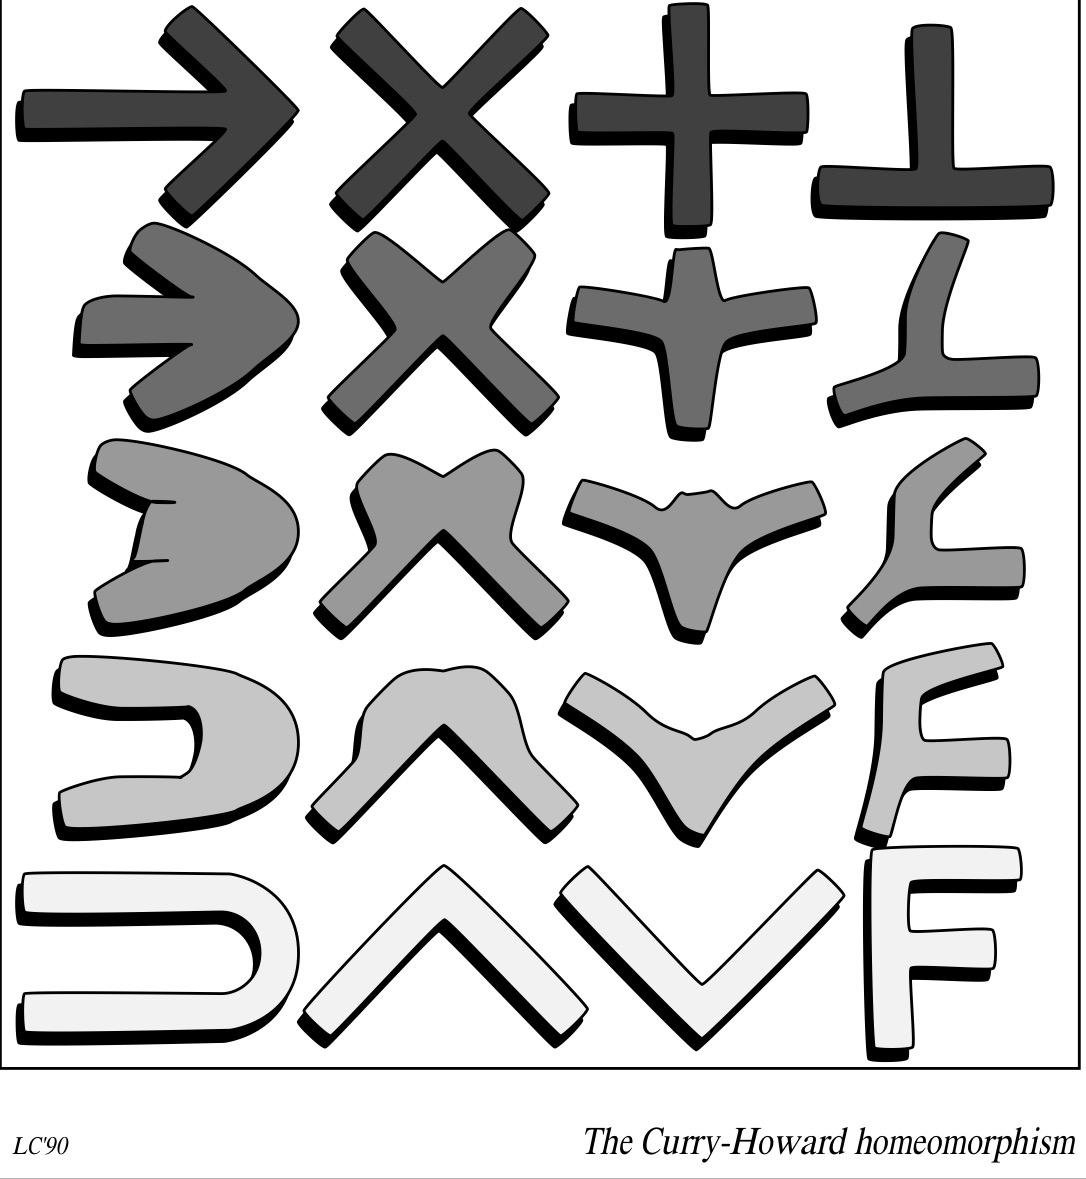
\includegraphics[scale=0.1]{cardelli-hc-corr.jpg}\\
      {\tiny Source: \url{http://lucacardelli.name/Artifacts/Drawings/CurryHoward/CurryHoward.pdf}}
    \end{figure}

\end{center}
\end{frame}

\begin{frame}[c]
  \frametitle{Background Work: Second Order Intuitionistic Propositional Logic}
  \begin{center}
    \uncover<2->{\LARGE {\color{red}Propositions are truth values not resources}}\\
    \uncover<1->{{\small
        \fbox{Language}
        \begin{flalign*}
          \text{Propostions \& connectives}\quad A, B, C &::= x \mid A \supset B \mid \forall x. B \mid ... \\
          \text{Context}\quad \Gamma,\Delta &::= \epsilon \mid \Gamma, A
        \end{flalign*}
        \fbox{Logic Rules}
        \begin{figure}[h]\centering
          % ID
          \begin{minipage}{0.20\linewidth}
            \begin{prooftree}
              \AxiomC{${\color{white}A \Gamma A}$}\RightLabel{[Ax]}
              \UnaryInfC{$A \vdash A $}
            \end{prooftree}
          \end{minipage}

          % \forall I
          \begin{minipage}{0.5\linewidth}
            \begin{prooftree}
              \AxiomC{$\Gamma \vdash B$}
              \AxiomC{$x \notin \Gamma$}\RightLabel{[$\forall$I]}
              \BinaryInfC{$\forall x. B$}
            \end{prooftree}
          \end{minipage}\hfill%
          % \forall E
          \begin{minipage}{0.5\linewidth}
            \begin{prooftree}
              \AxiomC{$\Gamma \vdash \forall x. B$}
              \AxiomC{$\Gamma \vdash A$}\RightLabel{[$\forall$E]}
              \BinaryInfC{$B[x/A]$}
            \end{prooftree}
          \end{minipage}

          % -> I
          \begin{minipage}{0.5\linewidth}
            \begin{prooftree}
              \AxiomC{$\Gamma,A \vdash B$}\RightLabel{[$\supset$I]}
              \UnaryInfC{$\Gamma \vdash A \supset B$}
            \end{prooftree}
          \end{minipage}\hfill%
          % -> E
          \begin{minipage}{0.5\linewidth}
            \begin{prooftree}
              \AxiomC{$\Gamma \vdash A \supset B$}
              \AxiomC{$\Gamma \vdash A$}\RightLabel{[$\supset$E]}
              \BinaryInfC{$\Gamma \vdash B $}
            \end{prooftree}
          \end{minipage}
        \end{figure}
      }
    }
  \end{center}
\end{frame}


\begin{frame}[c]
  \frametitle{Background Work: Substructural Logic}
  \begin{center}
    \begin{itemize}
    \item<1-> Structural rules implicit in intuitionistic propositional logics\\
      % WKN
      \begin{minipage}{0.33\linewidth}
        \begin{prooftree}
          \AxiomC{$\Gamma \vdash B$}\RightLabel{[WKN]}
          \UnaryInfC{$\Gamma, A \vdash B$}
        \end{prooftree}
      \end{minipage}\hfill%
      % CTR
      \begin{minipage}{0.33\linewidth}
        \begin{prooftree}
          \AxiomC{$\Gamma, A, A \vdash B$}\RightLabel{[CTR]}
          \UnaryInfC{$\Gamma, A \vdash B $}
        \end{prooftree}
      \end{minipage}\hfill%
      % EXCH
      \begin{minipage}{0.33\linewidth}
        \begin{prooftree}
          \AxiomC{$\Gamma, \Delta \vdash B$}\RightLabel{[EXCH]}
          \UnaryInfC{$\Delta, \Gamma \vdash B $}
        \end{prooftree}
      \end{minipage}

    \item <2-> Control the use of [WKN] and [CTR]\\
    \end{itemize}
    \uncover<2->{\LARGE \color{red} Propositions now behave like resources}
  \end{center}
\end{frame}

\begin{frame}[c]
  \frametitle{Background Work: Substructural Logic}
  \begin{center}
    \begin{tabular}[h]{c c c}
      System                                                    & Who    & Restrictions\\\hline\hline
      Linear Logic\citep{girard_linear_1987}                    & Girard & [WKN] [CTRN]\\
%      Revelance Logic                                           & Orlev  & \\
      Lambek Logic\citep{lambek_mathematics_1958}               & Lambek & [EXCH]\\
      Logic of Bunched Implications\citep{ohearn_logic_1999}    & O'Hearn and Pym & [WKN] [CTRN]\\
      \vdots                                                    & \vdots & \vdots 
    \end{tabular}
  \end{center}
\end{frame}


% \begin{frame}[c]
%   \frametitle{Background Work: Linear Logic}
%   Certain contexts cannot undergo weakening or contraction\citep{girard_linear_1987, wadler_taste_1993}\\
%   \begin{flalign*}
%     \text{Context}\quad \Gamma,\Delta &::= \epsilon \mid \Gamma, \Pair{A} \mid \Gamma, [A]
%   \end{flalign*}

%   \begin{flalign*}
%     \Gamma, \Pair{A} &\not\vdash \Gamma\\
%     \Gamma, \Pair{A} &\not\vdash \Gamma, \Pair{A}, \Pair{A}\\
%     \Gamma, [A] &\vdash \Gamma\\
%     \Gamma, [A] &\vdash \Gamma, [A], [A]\\
%   \end{flalign*}
% \end{frame}

% \begin{frame}
%   \frametitle{Background Work: Linear Logic}
%   \begin{center}
%   \fbox{Language}\\
%   \begin{flalign*}
%     \text{Context} \Gamma,\Delta &::= \epsilon \mid \Gamma, \Pair{A} \mid \Gamma, [A]\\
%     \text{Propostions} A, B, C &::= X \mid \oc A \mid A \rightspoon B \mid A \with B \mid A \otimes B \mid A \oplus B
%   \end{flalign*}
%   \fbox{Structural Rules}\\
%   \begin{figure}[h]
%   \centering
%  % []ID
%     \begin{minipage}{0.30\textwidth}
%       \begin{prooftree}
%         \AxiomC{{\color{white}$\Gamma, \Delta \vdash A$}} \RightLabel{[ID$_{[]}$]}
%         \UnaryInfC{$[A] \vdash A$}
%       \end{prooftree}
%     \end{minipage}
%   % !ID
%     \begin{minipage}{0.30\textwidth}
%       \begin{prooftree}
%         \AxiomC{{\color{white}$\Gamma, \Delta \vdash A$}} \RightLabel{[ID$_{\Pair{}}$]}
%         \UnaryInfC{$\Pair{A} \vdash A$}
%       \end{prooftree}
%     \end{minipage}

%     % EXCH
%     \begin{minipage}{0.30\textwidth}
%       \begin{prooftree}
%         \AxiomC{$\Gamma, \Delta \vdash A$} \RightLabel{[EXCH]}
%         \UnaryInfC{$\Delta, \Gamma \vdash A$}
%       \end{prooftree}
%     \end{minipage}
%     % CTRN
%     \begin{minipage}{0.30\textwidth}
%       \begin{prooftree}
%         \AxiomC{$\Gamma, [A], [A] \vdash B$} \RightLabel{[CTRN]}
%         \UnaryInfC{$\Gamma, [A] \vdash B$}
%       \end{prooftree}
%     \end{minipage}
%     % WKN
%     \begin{minipage}{0.30\textwidth}
%       \begin{prooftree}
%         \AxiomC{$\Gamma \vdash B$} \RightLabel{[WKN]}
%         \UnaryInfC{$\Gamma, [A] \vdash B$}
%       \end{prooftree}
%     \end{minipage}

%     % ! I
%     \begin{minipage}{0.30\textwidth}
%       \begin{prooftree}
%         \AxiomC{$[\Gamma] \vdash A$} \RightLabel{[$\oc$I]}
%         \UnaryInfC{$[\Gamma] \vdash \oc A$}
%       \end{prooftree}
%     \end{minipage}
%     % ! E
%     \begin{minipage}{0.30\textwidth}
%       \begin{prooftree}
%         \AxiomC{$\Gamma \vdash \oc A$}
%         \AxiomC{$\Delta, [A] \vdash B$} \RightLabel{[$\oc$E]}
%         \BinaryInfC{$\Gamma, \Delta \vdash B$}
%       \end{prooftree}
%     \end{minipage}
%   \end{figure}
% \end{center}
% \end{frame}

% \begin{frame}
%   \frametitle{Background Work: Linear Logic}
%   \begin{center}
%       \fbox{
%       Connective Rules
%     }
%     \begin{itemize}[\noindent {}]
%     \item[]<1->
%      % -o I
%     \begin{minipage}{0.30\textwidth}
%       \begin{prooftree}
%         \AxiomC{$\Gamma, A \vdash B$} \RightLabel{$[\rightspoon I]$}
%         \UnaryInfC{$\Gamma \vdash A \rightspoon B$}
%       \end{prooftree}
%     \end{minipage}\hfill%
%     % -o E
%     \begin{minipage}{0.60\textwidth}
%       \begin{prooftree}
%         \AxiomC{$\Gamma \vdash  A \rightspoon B$}
%         \AxiomC{$\Delta \vdash A$} \RightLabel{$[\rightspoon E]$}
%         \BinaryInfC{$\Gamma, \Delta \vdash B$}
%       \end{prooftree}
%     \end{minipage}
%     % & I
%     \item[]<2-> \begin{minipage}{.3\textwidth}
%       \begin{prooftree}
%         \AxiomC{$\Gamma \vdash A$}
%         \AxiomC{$\Gamma \vdash B$} \RightLabel{$[\with I]$}
%         \BinaryInfC{$\Gamma \vdash A \with B$}
%       \end{prooftree}
%     \end{minipage}\hfill%
%     % & E_1
%     \begin{minipage}{.3\textwidth}
%       \begin{prooftree}
%         \AxiomC{$\Gamma \vdash A \with B$} \RightLabel{$[\with E_1]$}
%         \UnaryInfC{$\Gamma \vdash A$}
%       \end{prooftree}
%     \end{minipage}\hfill%
%     % & E_2
%     \begin{minipage}{.3\textwidth}
%       \begin{prooftree}
%         \AxiomC{$\Gamma \vdash A \with B$} \RightLabel{$[\with E_2]$}
%         \UnaryInfC{$\Gamma \vdash B$}
%       \end{prooftree}
%     \end{minipage}
%   \item[]<3->
%     % otimes I
%     \begin{minipage}{.3\textwidth}
%       \begin{prooftree}
%         \AxiomC{$\Gamma \vdash A$}
%         \AxiomC{$\Delta \vdash B$} \RightLabel{$[\otimes I]$}
%         \BinaryInfC{$\Gamma, \Delta \vdash A \otimes B$}
%       \end{prooftree}
%     \end{minipage}\hfill%
%     % otimes E
%     \begin{minipage}{.6\textwidth}
%       \begin{prooftree}
%         \AxiomC{$\Gamma \vdash A \otimes B$} \RightLabel{$[\otimes E]$}
%         \AxiomC{$\Delta, A, B \vdash C$}
%         \BinaryInfC{$\Gamma,\Delta \vdash C$}
%       \end{prooftree}
%     \end{minipage}
%   \item[]<4->
%     % oplus I_1
%     \begin{minipage}{.45\textwidth}
%       \begin{prooftree}
%         \AxiomC{$\Gamma \vdash A$} \RightLabel{$[\oplus I_1]$}
%         \UnaryInfC{$\Gamma \vdash A \oplus B$}
%       \end{prooftree}
%     \end{minipage}\hfill%
%     % oplus I_1
%     \begin{minipage}{.45\textwidth}
%       \begin{prooftree}
%         \AxiomC{$\Delta \vdash B$} \RightLabel{$[\oplus I_2]$}
%         \UnaryInfC{$\Delta \vdash A \oplus B$}
%       \end{prooftree}
%     \end{minipage}
%     % oplus E
%     \begin{minipage}{1\textwidth}
%       \begin{prooftree}
%         \AxiomC{$\Gamma \vdash A \oplus B$}
%         \AxiomC{$\Delta, A \vdash C$}
%         \AxiomC{$\Delta, B \vdash C$}\RightLabel{$[\oplus E]$}
%         \TrinaryInfC{$\Gamma, \Delta \vdash C$}
%       \end{prooftree}
%     \end{minipage}
%   \end{itemize}
%   \end{center}
% \end{frame}

% \begin{frame}[fragile,c]
%   \frametitle{Background Work: Linear Logic}
%   \begin{itemize}
%   \item<1-> Propositions act like Resources\\
%     \begin{center}
%       ``A consumed to give B''\quad $A, A \rightspoon B \vdash B$\\
%       ``Both A and B''\quad $A \otimes B$\\
%       ``Choice between A and B''\quad $A \with B$\\
%     Cannot create new copies\quad $A \not\vdash A \otimes A$\\
%     %\[
%       %\bigpumpkin%, \bigpumpkin \rightspoon \mathcloud \vdash \mathcloud
%     %\]
%     Fall back to intuitionistic logic\quad $\oc A \rightspoon B \equiv A \supset B$
%   \end{center}
%   \item<2-> Curry-Howard Correspondence: Type systems based on Linear Logic
%   \item<2-> Active Area of research: L$^3$\citep{ahmed_l3_2007},
%     F$^\circ$\citep{mazurak_lolliproc_2010}, Linear Haskell\citep{bernardy_linear_2017}, Quill\citep{morris_best_2016}
%   \item<2-> Resources are first class values
%   \end{itemize}
% \end{frame}

% \begin{frame}[fragile, c]
%   \frametitle{Background Work: Linear Logic}
%   Downside: Asymmetry between implication and conjunction\\
%   Multiplicative Fragment:
%   \begin{center}
%     $$A \otimes B \vdash C \text{ iff } A \vdash B \rightspoon C$$
%   \end{center}
%   Additive Fragment:
%   \begin{center}
%     $$ \oc A \with \oc B \vdash C \text{ iff } \oc A \vdash \oc B \rightspoon C$$
%   \end{center}
%   Modality is necessary to avoid over-restriction
% \end{frame}

\begin{frame}[c]
  \frametitle{Background Work: Logic of Bunched Implications (\BI{})}
  \begin{center}
    \begin{itemize}
  \item Contexts are usually lists or sets
    $$ \Gamma, A, B $$
  \item In logic of \BI{}, contexts are trees and called are bunches
  \item Two connective used to combine bunches: $A;B$ or $A, B$\\
    \begin{center}
      \begin{figure}[h]\centering
      \begin{minipage}{0.5\linewidth}\centering
        \tikzset{every tree node/.style={minimum width=2em},
          blank/.style={draw=none},
          edge from parent/.style=
          {draw,edge from parent path={(\tikzparentnode) -- (\tikzchildnode)}},
          level distance=1.5cm}
        \begin{tikzpicture}
          \Tree
          [.,
          [.;
          [.A ]
          [.B ]
          ]
          [.C ]
          ]
        \end{tikzpicture}
        \caption*{$\Gamma = (A;B),C$}
      \end{minipage}%
      \begin{minipage}{0.5\linewidth}\centering
        \tikzset{every tree node/.style={minimum width=2em},
          blank/.style={draw=none},
          edge from parent/.style=
          {draw,edge from parent path={(\tikzparentnode) -- (\tikzchildnode)}},
          level distance=1.5cm}
        \begin{tikzpicture}
          \Tree
          [.;
          [.A ]
          [.,
          [.C ]
          [.B ]
          ]
          ]
        \end{tikzpicture}
        \caption*{$\Gamma = A;(B,C)$}
      \end{minipage}
    \end{figure}

    \end{center}

\end{itemize}
\end{center}
\end{frame}

\begin{frame}[c]
  \frametitle{Background Work: Logic of \BI{}}
  \begin{center}
  Structural rules guided by context connectives

  \begin{itemize}
  \item Weakening
    \begin{center}
      $A \vdash A;A$\\
      $A \not\vdash A,A$
    \end{center}

  \item Contraction
    \begin{center}
      $A;A \vdash A$ \qquad $A;B \vdash B$\\
      $A,B \not\vdash A$ \qquad $A,B \not\vdash B$
    \end{center}
  \end{itemize}

  Interpretation:
  \begin{itemize}
  \item Propositions connected with , are separate resources
  \item Propositions connected with ; are sharing resources
\end{itemize}
\end{center}

\end{frame}

\begin{frame}[c]
  \frametitle{Background Work: Logic of \BI{}}
  \begin{center}
    (Absence of) Structural rules and logical connectives:
    \begin{itemize}
    \item Meaning of conjunction
      \begin{center}
      \begin{minipage}{0.45\linewidth}
        \begin{flalign*}
          A,B \vdash A \otimes B
        \end{flalign*}
      \end{minipage}\hfill%
      \begin{minipage}{0.45\linewidth}
        \begin{flalign*}
        A;B \vdash A \with B
      \end{flalign*}
      \end{minipage}
    \end{center}
    \item Meaning of implication
      \begin{minipage}{0.5\linewidth}
        \begin{prooftree}
          \AxiomC{$\Gamma, A \vdash B$} \RightLabel{[$\sepimp$I]}
          \UnaryInfC{$\Gamma \vdash A \sepimp B$}
        \end{prooftree}
      \end{minipage}%
      \begin{minipage}{0.5\linewidth}
        \begin{prooftree}
          \AxiomC{$\Gamma; A \vdash B$} \RightLabel{[$\shimp$I]}
          \UnaryInfC{$\Gamma \vdash A \shimp B$}
        \end{prooftree}
      \end{minipage}
    \end{itemize}
  \end{center}
\end{frame}


\begin{frame}
  \frametitle{Background work: Logic of \BI{}}
  \begin{center}
    Coffee Shop

    1 cup coffee costs \$2

    \uncover<1->{
      \begin{tabular}[c]{c c c c c}
        \raisebox{-0.4\height}{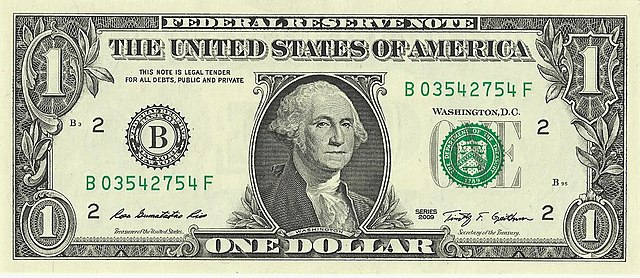
\includegraphics[scale=0.205]{one_usd}}
        & {\LARGE $\otimes$}
        & \raisebox{-0.4\height}{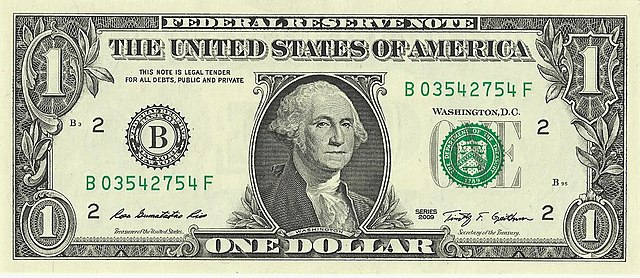
\includegraphics[scale=0.205]{one_usd}}
        & {\LARGE $\vdash$}
        & \raisebox{-0.4\height}{
\includegraphics[scale=0.03]{coffee_cup}}
      \end{tabular}
    }
    \uncover<2->{
      \begin{tabular}[c]{c c c c c}
        \raisebox{-0.4\height}{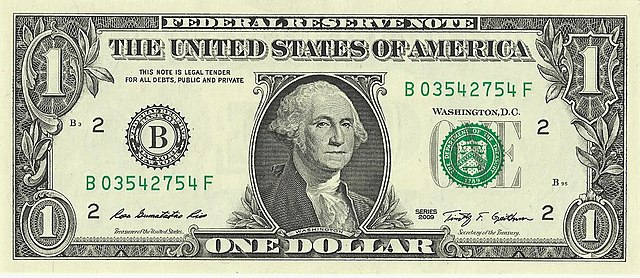
\includegraphics[scale=0.2]{one_usd}}
        & {\LARGE $\with$}
        & \raisebox{-0.4\height}{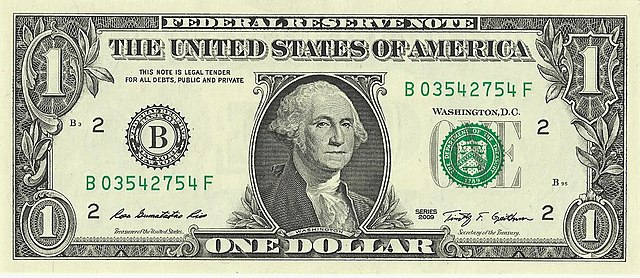
\includegraphics[scale=0.2]{one_usd}}
        & {\LARGE $\not\vdash$}
        & \raisebox{-0.4\height}{
\includegraphics[scale=0.03]{coffee_cup}}
      \end{tabular}
    }
  \end{center}
\end{frame}


\begin{frame}
  \frametitle{Background work: Logic of \BI{}}
  \begin{center}
    Coffee Shop

    1 cup coffee costs \$2

    \begin{tabular}[c]{c c c c c}
      \raisebox{-0.4\height}{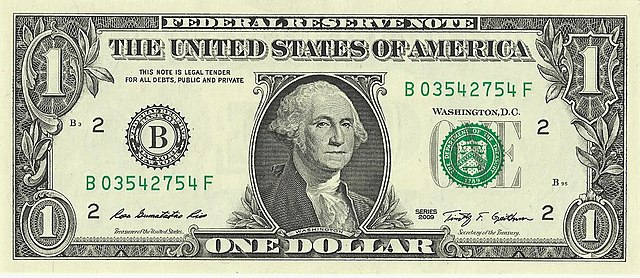
\includegraphics[scale=0.205]{one_usd}}
      & {\LARGE $\vdash$}
      & \raisebox{-0.4\height}{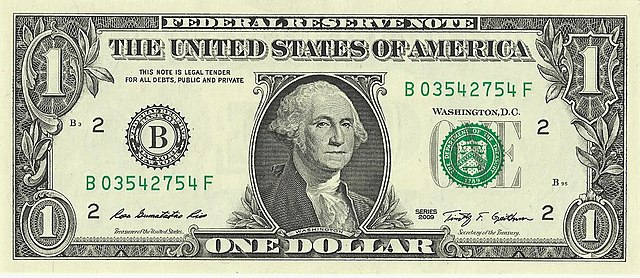
\includegraphics[scale=0.2]{one_usd}}
      & {\LARGE $\sepimp$}
      & \raisebox{-0.4\height}{
\includegraphics[scale=0.03]{coffee_cup}}
    \end{tabular}
    \begin{tabular}[c]{c c c c c c c}
      \raisebox{-0.4\height}{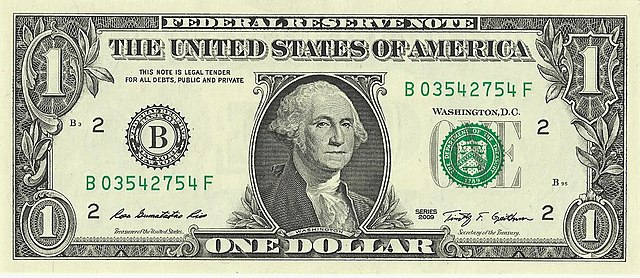
\includegraphics[scale=0.15]{one_usd}}
      & {\LARGE $;$}
      & \raisebox{-0.4\height}{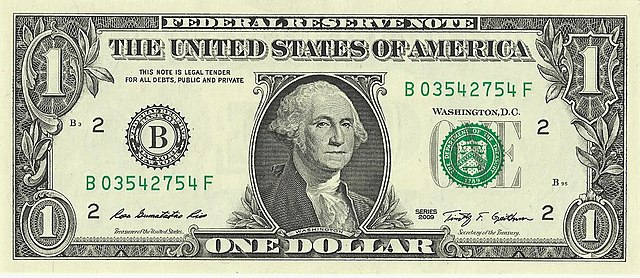
\includegraphics[scale=0.15]{one_usd}}
      & {\LARGE $\sepimp$}
      & \raisebox{-0.4\height}{
\includegraphics[scale=0.015]{coffee_cup}}
      & {\LARGE $\not\vdash$}
      & \raisebox{-0.4\height}{
\includegraphics[scale=0.015]{coffee_cup}}
    \end{tabular}
  \end{center}
\end{frame}


% \begin{frame}[c]
%   \frametitle{Background Work: Typing Rules with Qualified Types}
%   \HM{} system with qualified Types:
%   \begin{figure}[h]
%     \centering
%     {\small
%       \begin{minipage}{.35\textwidth}
%       \begin{prooftree}
%         \AxiomC{$x: \sigma \in \Gamma$} \RightLabel{[VAR]}
%         \UnaryInfC{$P \mid \Gamma \vdash x : \sigma $}
%       \end{prooftree}
%     \end{minipage}%
%     % let
%     \begin{minipage}{.55\textwidth}
%       \begin{prooftree}
%         \AxiomC{$P \mid \Gamma \vdash M : \sigma$}
%         \AxiomC{$Q \mid \Gamma_{x}, x: \sigma \vdash N: \tau$} \RightLabel{[LET]}
%         \BinaryInfC{$P,Q \mid \Gamma \vdash (\Let{x}{M}{N}) : \tau$}
%       \end{prooftree}
%     \end{minipage}

%     % forall I
%     \begin{minipage}{0.55\textwidth}
%       \begin{prooftree}
%         \AxiomC{$P \mid \Gamma \vdash M : \sigma$}\RightLabel{[$\forall$ I]}
%         \AxiomC{$t \notin \texttt{fvs}(\Gamma) \cup \texttt{fvs}(P)$}
%         \BinaryInfC{$P \mid \Gamma \vdash M : \forall t. \sigma$}
%       \end{prooftree}
%     \end{minipage}%
%     % forall E
%     \begin{minipage}{0.40\textwidth}
%       \begin{prooftree}
%         \AxiomC{$P \mid \Gamma \vdash M : \forall t. \sigma$}\RightLabel{[$\forall$ E]}
%         \UnaryInfC{$P \mid \Gamma \vdash M: [\tau / t] \sigma$}
%       \end{prooftree}
%     \end{minipage}

%     % -> I
%     \begin{minipage}{0.40\textwidth}
%       \begin{prooftree}
%         \AxiomC{$P \mid \Gamma_{x}, x: \tau \vdash M : \tau'$} \RightLabel{[$\rightarrow$ I]}
%         \UnaryInfC{$P \mid \Gamma \vdash \lambda x. M : \tau \rightarrow \tau'$}
%       \end{prooftree}
%     \end{minipage}%
%     % -> E
%     \begin{minipage}{0.55\textwidth}
%       \begin{prooftree}
%         \AxiomC{$P \mid \Gamma \vdash M : \tau \rightarrow \tau'$}
%         \AxiomC{$P \mid \Gamma \vdash N : \tau$} \RightLabel{[$\rightarrow$ E]}
%         \BinaryInfC{$P \mid \Gamma \vdash M N : \tau'$}
%       \end{prooftree}
%     \end{minipage}

%     % => I
%     \begin{minipage}{0.40\textwidth}
%       {\color{red}
%         \begin{prooftree}
%           \AxiomC{$P, \pi \mid \Gamma \vdash M : \rho$} \RightLabel{[$\Rightarrow$I]}
%           \UnaryInfC{$P \mid \Gamma \vdash M : \pi \Rightarrow \rho$}
%         \end{prooftree}
%       }
%       \begin{center}
%       $\pi \Rightarrow \rho$: $\pi$ qualifies $\rho$
%     \end{center}

%     \end{minipage}%
%     % => E
%     \begin{minipage}{0.45\textwidth}
%       {\color{red}
%         \begin{prooftree}
%           \AxiomC{$P \mid \Gamma \vdash M : \pi \Rightarrow \rho$}
%           \AxiomC{$P \Rightarrow \pi$} \RightLabel{[$\Rightarrow$E]}
%           \BinaryInfC{$P \mid \Gamma \vdash M: \rho$}
%         \end{prooftree}
%       }
%       \begin{center}
%       $P \Rightarrow \pi$: $P$ entails $\pi$
%     \end{center}

%     \end{minipage}
%   }
% \end{figure}
% \begin{center}
% \qquad\qquad
% \end{center}
% \end{frame}


% \begin{frame}[fragile, c]
%   \frametitle{Background Work: $\alpha\lambda$-calculus}
%   Curry-Howard interpretation of logic of \BI{}\citep{ohearn_bunched_2003}\\
%   \begin{centering}
%   \fbox{Language}
%   \begin{flalign*}
%    \text{Context}\ \ \ \Gamma, \Delta &::= \{\}_m \mid \{\}_a \mid x:\tau \mid \Gamma, \Delta \mid \Gamma;\Delta\\
%     \text{Types}\ \ \  \tau, \upsilon &::= t \mid \iota \mid \tau \shimp \tau \mid \tau \sepimp \tau \\
%     \text{Expressions}\ \ \ M, N      &::= x \mid \lambda x. M \mid \alpha x. M \mid M N
%   \end{flalign*}
%   \fbox{Typing rules}
% \begin{figure}[h]
%   \centering
%     % var
%     \begin{minipage}{0.30\textwidth}
%       \begin{prooftree}
%         \AxiomC{$x: \tau \in \Gamma$} \RightLabel{[VAR]}
%         \UnaryInfC{$\Gamma \vdash x : \tau $}
%       \end{prooftree}
%     \end{minipage}%
%     % CTR
%     \begin{minipage}{0.30\textwidth}
%       \begin{prooftree}
%         \AxiomC{$\Gamma; \Gamma \vdash M:\tau$} \RightLabel{[CTR]}
%         \UnaryInfC{$\Gamma \vdash M:\tau$}
%       \end{prooftree}
%     \end{minipage}%
%     % WKN
%     \begin{minipage}{0.30\textwidth}
%       \begin{prooftree}
%         \AxiomC{$\Gamma \vdash M:\tau$} \RightLabel{[WKN]}
%         \UnaryInfC{$\Gamma;\Delta \vdash M:\tau $}
%       \end{prooftree}
%     \end{minipage}

%     % -* I
%     \begin{minipage}{0.45\textwidth}
%       \begin{prooftree}
%         \AxiomC{$\Gamma_{x}, x: \tau \vdash M : \tau'$} \RightLabel{[$\sepimp$I]}
%         \UnaryInfC{$\Gamma \vdash \lambda  x. M : \tau \sepimp \tau'$}
%       \end{prooftree}
%     \end{minipage}%
%     % -* E
%     \begin{minipage}{0.45\textwidth}
%       \begin{prooftree}
%         \AxiomC{$\Gamma \vdash M : \tau \sepimp \tau' \ \ \ \ \
%           \Delta \vdash N : \tau$} \RightLabel{[$\sepimp$E]}
%         \UnaryInfC{$\Gamma,\Delta \vdash M N : \tau'$}
%       \end{prooftree}
%     \end{minipage}

%     % -> I
%     \begin{minipage}{0.45\textwidth}
%       \begin{prooftree}
%         \AxiomC{$\Gamma_{x}; x: \tau \vdash M : \tau'$} \RightLabel{[$\shimp$I]}
%         \UnaryInfC{$\Gamma \vdash \alpha  x. M : \tau \shimp \tau'$}
%       \end{prooftree}
%     \end{minipage}%
%     % -> E
%     \begin{minipage}{0.45\textwidth}
%       \begin{prooftree}
%         \AxiomC{$\Gamma \vdash M : \tau \shimp \tau' \ \ \ \ \
%           \Delta \vdash N : \tau$} \RightLabel{[$\shimp$E]}
%         \UnaryInfC{$\Gamma;\Delta \vdash M N : \tau'$}
%       \end{prooftree}
%     \end{minipage}
% \end{figure}
% \end{centering}
% \end{frame}


%%% Local Variables:
%%% mode: latex
%%% TeX-master: "defense-slides"
%%% End:
